%!TEX root = ../../book_ML.tex
\chapter{Cơ sở lý thuyết}
\label{cha: chap2}
% \index{principal component analysis}
% \index{PCA -- \textit{xem} principle component analysis}
% \index{PCA}

% \index{phân tích thành phần chính -- principle component analysis}
% \index{principle component analysis -- phân tích thành phần chính}
% \index{PCA}
\section{Tổng quan về các kĩ thuật nén mất mát thông tin}

\section{Các kĩ thuật nén codec thường được sử dụng}

\section{Bộ mã hóa tự động (Autoencoder)}

Bộ mã hóa tự động là một kỹ thuật học tập không có giám sát,
trong đó chúng em tận dụng mạng nơ-ron cho nhiệm vụ của học để biểu diễn các tập
giá trị dưới dạng nén, học cách để giải mã dữ liệu từ dạng nén.

Cụ thể, chúng em sẽ thiết kế một kiến trúc mạng nơ-ron nhân tạo sau đó áp đặt một
nút thắt cổ chai trong mạng - điều này đại diện cho sự nén lại một cách tự động.
Mạng này sẽ phải biểu diễn tri thức đầu vào dưới dạng các biểu diễn trong ít
chiều không gian hơn, đây chính là biểu diễn nén của đầu vào.

\begin{figure}
    \begin{subfigure}{1.\textwidth}
        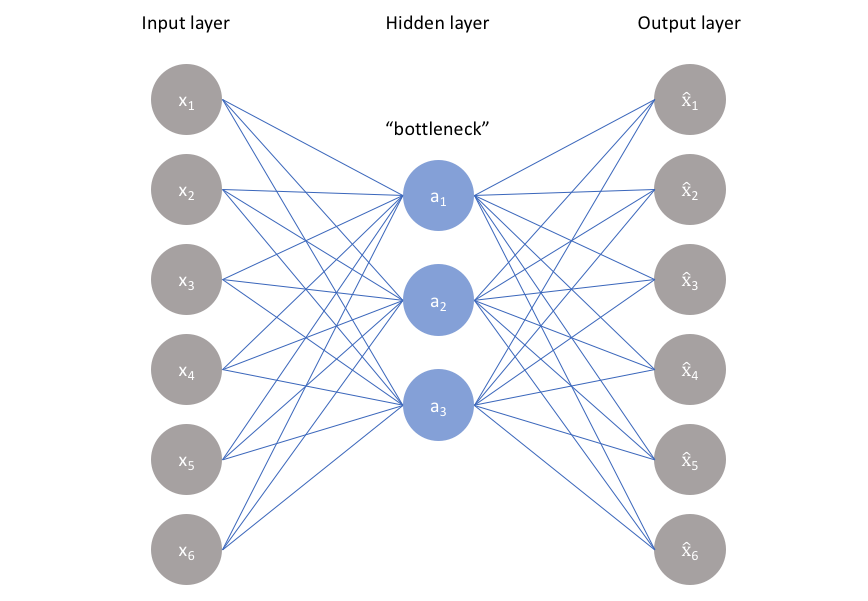
\includegraphics[width=1.\linewidth]{Chapters/items/autoencoder1.png}
        \caption{}
        \label{fig: auto1}
    \end{subfigure}
    \caption{Cấu trúc các phần của OpenCV.}
\end{figure}

\newpage
Nếu các tính năng đầu vào từng độc lập của nhau, việc nén này và tái tạo sau đó sẽ là
một nhiệm vụ rất khó khăn. Tuy nhiên, nếu một số loại cấu trúc tồn tại trong dữ liệu
(ví dụ như: mối tương quan giữa các tính năng đầu vào), cấu trúc này có thể được
học và do đó được tận dụng khi buộc đầu vào thông qua nút thắt cổ chai của mạng.

Bộ mã hóa tự động lý tưởng cân bằng những điều sau đây:
\begin{itemize}
    \item Nhạy cảm với các yếu tố đầu vào đủ để xây dựng lại một cách chính xác.
    \item Đủ nhạy cảm với các đầu vào mà mô hình không chỉ đơn giản là ghi
          nhớ hoặc trang bị quá nhiều dữ liệu đào tạo.
\end{itemize}

\newpage
Sự đánh đổi này buộc mô hình chỉ duy trì các biến thể trong dữ liệu cần
thiết để cấu trúc lại đầu vào mà không giữ lại các phần dư thừa trong đầu vào.
Đối với hầu hết các trường hợp, điều này liên quan đến việc xây dựng một hàm mất mát
trong đó phải thỏa mãn mô hình của chúng ta nhạy cảm với các yếu tố đầu vào
(ví dụ: xây dựng lại 1 hàm mất mát ${\cal L}\left( {x,\hat x} \right)$ và
thêm một chính quy hóa)


\begin{equation}
    {\cal L}\left( {x,\hat x} \right) + regularizer
\end{equation}

Thông thường, sẽ có thêm một tham số tỷ lệ trước thuật ngữ chính quy để chúng ta
có thể điều chỉnh sự cân bằng giữa hai mục tiêu.

Dưới đây chúng em sẽ trình bày về một số kiến trúc của bộ mã hóa tư động
tiêu chuẩn để áp đặt 2 ràng buộc này và điều chỉnh sự cân bằng.


% \newpage
% \subsection{Cấu trúc bộ mã hóa tự động}
% Một bộ mã hóa tự động có 3 thành phần chính : bộ mã hóa f,
% bộ giải mã g, mô hình xác suất Q

\subsection{Bộ mã hóa tự động chưa hoàn chỉnh}

Kiến trúc đơn giản nhất để xây dựng bộ mã tự động là hạn chế số lượng
nút hiện diện trong (các) lớp ẩn của mạng, hạn chế lượng thông tin có
thể truyền qua mạng. Bằng cách sử dụng các hình phạt mạng theo lỗi xây dựng lại,
mô hình của chúng tôi có thể tìm hiểu các thuộc tính quan trọng nhất của dữ
liệu đầu vào và cách tái tạo tốt nhất dữ liệu đầu vào ban đầu từ trạng thái
"được mã hóa". Lý tưởng nhất là bảng mã này sẽ tìm hiểu và mô tả các thuộc
tính tiềm ẩn của dữ liệu đầu vào.



